\documentclass[crop,tikz]{standalone}
\usepackage[T1]{fontenc}
\usepackage{tikz}
\usetikzlibrary{matrix,backgrounds,arrows.meta,fit,positioning,decorations.pathreplacing}
\begin{document}

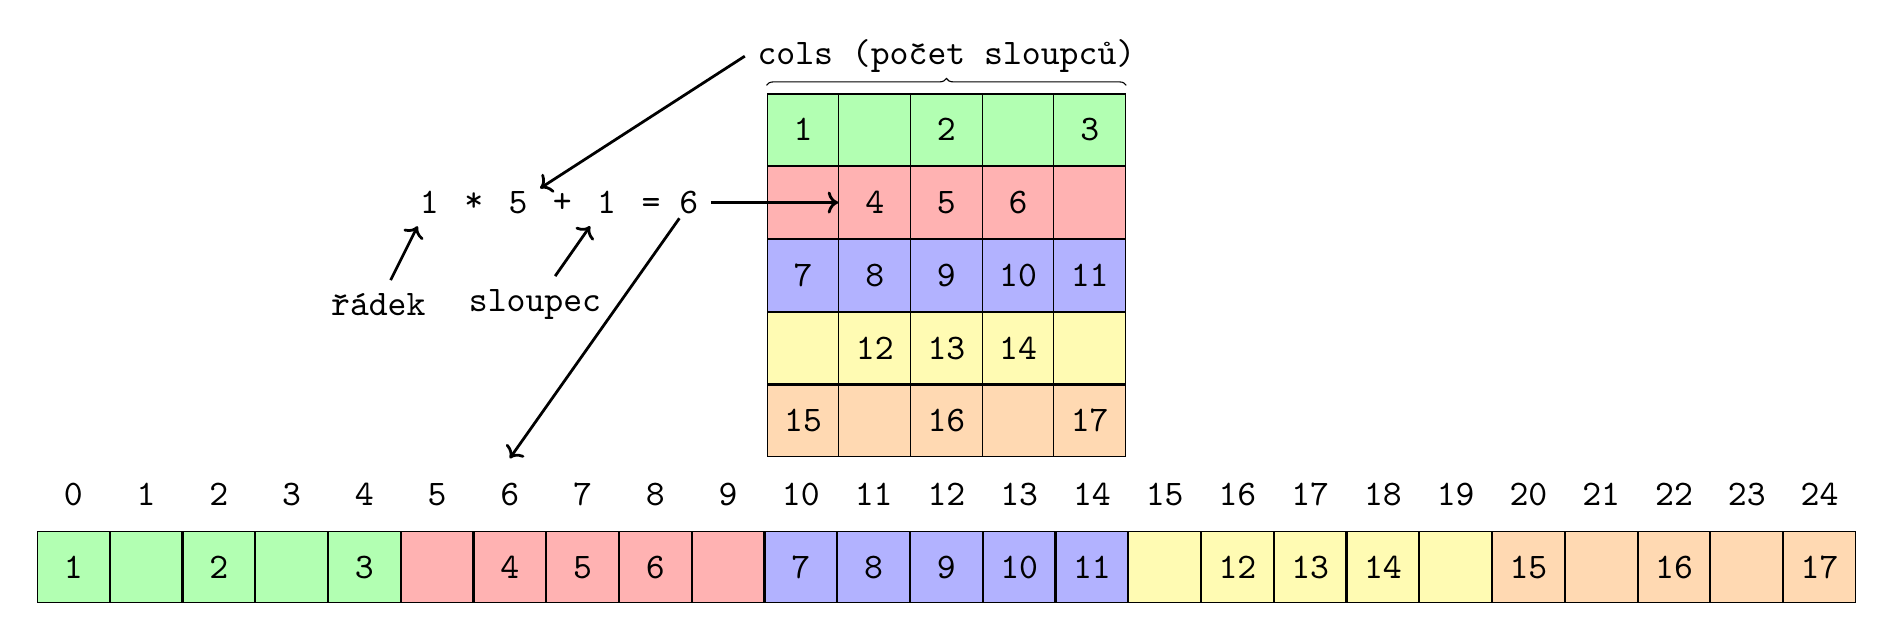
\begin{tikzpicture}[font=\ttfamily,every node/.style={scale=1.3},
  array/.style={nodes={draw, minimum size=7mm, anchor=center,fill=green!30},column sep=-\pgflinewidth, row sep=0mm},
	linearray/.style={nodes={draw, minimum size=7mm}}
]




\matrix[array] (array)  {

	
	
		\node[fill=green!30] (array-1-1) { 1 }; &
	
		\node[fill=green!30] (array-1-2) {   }; &
	
		\node[fill=green!30] (array-1-3) { 2 }; &
	
		\node[fill=green!30] (array-1-4) {   }; &
	
		\node[fill=green!30] (array-1-5) { 3 }; 
	 \\

	
	
		\node[fill=red!30] (array-2-1) {   }; &
	
		\node[fill=red!30] (array-2-2) { 4 }; &
	
		\node[fill=red!30] (array-2-3) { 5 }; &
	
		\node[fill=red!30] (array-2-4) { 6 }; &
	
		\node[fill=red!30] (array-2-5) {   }; 
	 \\

	
	
		\node[fill=blue!30] (array-3-1) { 7 }; &
	
		\node[fill=blue!30] (array-3-2) { 8 }; &
	
		\node[fill=blue!30] (array-3-3) { 9 }; &
	
		\node[fill=blue!30] (array-3-4) { 10 }; &
	
		\node[fill=blue!30] (array-3-5) { 11 }; 
	 \\

	
	
		\node[fill=yellow!30] (array-4-1) {   }; &
	
		\node[fill=yellow!30] (array-4-2) { 12 }; &
	
		\node[fill=yellow!30] (array-4-3) { 13 }; &
	
		\node[fill=yellow!30] (array-4-4) { 14 }; &
	
		\node[fill=yellow!30] (array-4-5) {   }; 
	 \\

	
	
		\node[fill=orange!30] (array-5-1) { 15 }; &
	
		\node[fill=orange!30] (array-5-2) {   }; &
	
		\node[fill=orange!30] (array-5-3) { 16 }; &
	
		\node[fill=orange!30] (array-5-4) {   }; &
	
		\node[fill=orange!30] (array-5-5) { 17 }; 
	 \\

 \\ };

\matrix[linearray] (arrayline) [below of=array,yshift=-15mm] {

	
	
		\node[draw=none] (linearray-idx-1-1) { 0 }; &
	
		\node[draw=none] (linearray-idx-1-2) { 1 }; &
	
		\node[draw=none] (linearray-idx-1-3) { 2 }; &
	
		\node[draw=none] (linearray-idx-1-4) { 3 }; &
	
		\node[draw=none] (linearray-idx-1-5) { 4 }; &
	 

	
	
		\node[draw=none] (linearray-idx-2-1) { 5 }; &
	
		\node[draw=none] (linearray-idx-2-2) { 6 }; &
	
		\node[draw=none] (linearray-idx-2-3) { 7 }; &
	
		\node[draw=none] (linearray-idx-2-4) { 8 }; &
	
		\node[draw=none] (linearray-idx-2-5) { 9 }; &
	 

	
	
		\node[draw=none] (linearray-idx-3-1) { 10 }; &
	
		\node[draw=none] (linearray-idx-3-2) { 11 }; &
	
		\node[draw=none] (linearray-idx-3-3) { 12 }; &
	
		\node[draw=none] (linearray-idx-3-4) { 13 }; &
	
		\node[draw=none] (linearray-idx-3-5) { 14 }; &
	 

	
	
		\node[draw=none] (linearray-idx-4-1) { 15 }; &
	
		\node[draw=none] (linearray-idx-4-2) { 16 }; &
	
		\node[draw=none] (linearray-idx-4-3) { 17 }; &
	
		\node[draw=none] (linearray-idx-4-4) { 18 }; &
	
		\node[draw=none] (linearray-idx-4-5) { 19 }; &
	 

	
	
		\node[draw=none] (linearray-idx-5-1) { 20 }; &
	
		\node[draw=none] (linearray-idx-5-2) { 21 }; &
	
		\node[draw=none] (linearray-idx-5-3) { 22 }; &
	
		\node[draw=none] (linearray-idx-5-4) { 23 }; &
	
		\node[draw=none] (linearray-idx-5-5) { 24 }; &
	 
 \\


	
	
		\node[fill=green!30] (linearray-1-1) { 1 }; &
	
		\node[fill=green!30] (linearray-1-2) {   }; &
	
		\node[fill=green!30] (linearray-1-3) { 2 }; &
	
		\node[fill=green!30] (linearray-1-4) {   }; &
	
		\node[fill=green!30] (linearray-1-5) { 3 }; &
	

	
	
		\node[fill=red!30] (linearray-2-1) {   }; &
	
		\node[fill=red!30] (linearray-2-2) { 4 }; &
	
		\node[fill=red!30] (linearray-2-3) { 5 }; &
	
		\node[fill=red!30] (linearray-2-4) { 6 }; &
	
		\node[fill=red!30] (linearray-2-5) {   }; &
	

	
	
		\node[fill=blue!30] (linearray-3-1) { 7 }; &
	
		\node[fill=blue!30] (linearray-3-2) { 8 }; &
	
		\node[fill=blue!30] (linearray-3-3) { 9 }; &
	
		\node[fill=blue!30] (linearray-3-4) { 10 }; &
	
		\node[fill=blue!30] (linearray-3-5) { 11 }; &
	

	
	
		\node[fill=yellow!30] (linearray-4-1) {   }; &
	
		\node[fill=yellow!30] (linearray-4-2) { 12 }; &
	
		\node[fill=yellow!30] (linearray-4-3) { 13 }; &
	
		\node[fill=yellow!30] (linearray-4-4) { 14 }; &
	
		\node[fill=yellow!30] (linearray-4-5) {   }; &
	

	
	
		\node[fill=orange!30] (linearray-5-1) { 15 }; &
	
		\node[fill=orange!30] (linearray-5-2) {   }; &
	
		\node[fill=orange!30] (linearray-5-3) { 16 }; &
	
		\node[fill=orange!30] (linearray-5-4) {   }; &
	
		\node[fill=orange!30] (linearray-5-5) { 17 }; &
	

 \\ };


\node[left=4cm of array-2-1.west] (idx_row) {1};
\node[right=0cm of idx_row] (idx_mul) {*};
\node[right=0cm of idx_mul] (idx_cols) {5};
\node[right=0cm of idx_cols] (idx_add) {+};
\node[right=0cm of idx_add] (idx_col) {1};
\node[right=0cm of idx_col] (idx_res) {= 6};

% result to matrices
\draw[->,line width=1pt] (idx_res) -> (array-2-2.west);
\draw[->,line width=1pt] ([xshift=-4mm,yshift=-2mm]idx_res.east) -> (linearray-idx-2-2.north);

% cols
\draw[decoration={brace},decorate]([yshift=+1mm]array-1-1.north west) -- node[above] (cols) {cols (počet sloupců)} ([yshift=+1mm]array-1-5.north east);
\draw[->,line width=1pt] (cols.west) -> (idx_cols);

% rows, cols arrows
\draw[->,line width=1pt] node[below of=idx_row,xshift=-5mm] {řádek} edge (idx_row);
\draw[->,line width=1pt] node[below of=idx_col,xshift=-7mm] {sloupec} edge (idx_col);


\end{tikzpicture}


\end{document}
